\subsection{Primo sprint}

\begin{minipage}{\textwidth}
Di seguito è riportata la distribuzione delle ore per ciascun membro del team, accumulate in totali per persona e per ruolo:
\begin{table}[H]
  \begin{tabularx}{\textwidth}{|c|*{6}{>{\centering}X|}c|}
    \hline
    \multicolumn{8}{|c|}{\textbf{Consuntivo orario}} \\
    \hline
    \textbf{Membro del team} & \textbf{Re} & \textbf{Am} & \textbf{An} & \textbf{Pt} & \textbf{Pr} & \textbf{Ve} & \textbf{Totale per persona} \\
    \hline
    Cavalli Riccardo & 7 & 0 & 0 & 0 & 0 & 0 & 7 \\
    \hline
    Pianon Raul & 0 & 0 & 0 & 0 & 0 & 8 & 8 \\
    \hline
    Dall'Amico Martina & 0 & 0 & 8 & 0 & 0 & 0 & 8 \\
    \hline
    Cristo Marco & 0 & 0 & 7 & 0 & 0 & 0 & 7 \\
    \hline
    Lewental Sebastiano & 0 & 0 & 7 & 0 & 0 & 0 & 7 \\
    \hline
    Zecchinato Mattia & 0 & 0 & 1 & 6 & 0 & 0 & 7 \\
    \hline
    Stocco Tommaso & 0 & 6 & 0 & 0 & 0 & 0 & 6 \\
    \hline
    \textbf{Totale per ruolo} & 7 & 6 & 23 & 6 & 0 & 8 & \textbf{50} \\
    \hline
  \end{tabularx}
  \caption{Sprint 1 - Consuntivo orario}
\end{table}
\end{minipage}

\begin{figure}[H]
  \centering
  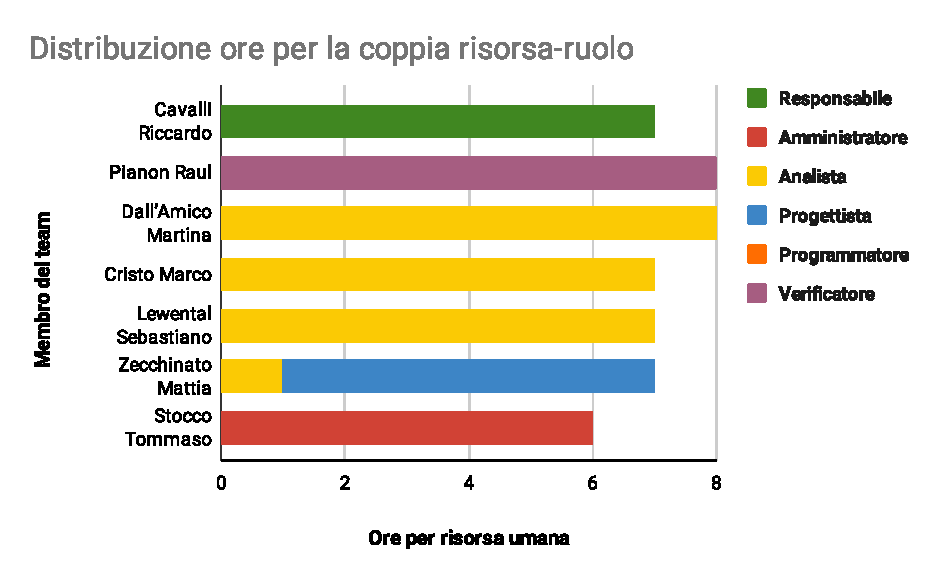
\includegraphics[width=0.90\textwidth]{assets/Consuntivo/Sprint-1/distribuzione_ore_risorsa_ruolo.pdf}
  \caption{Sprint 1 - Istogramma della distribuzione oraria per la coppia risorsa-ruolo}
\end{figure}

\begin{figure}[H]
  \centering
  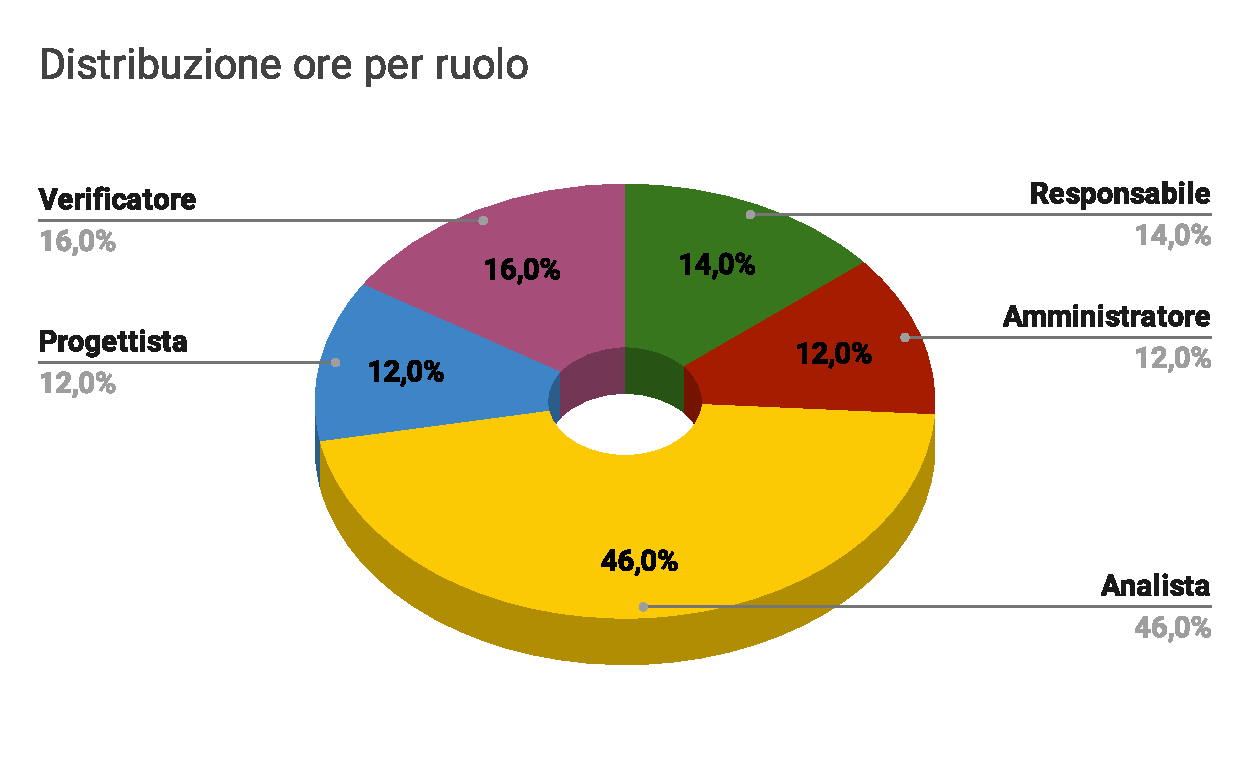
\includegraphics[width=0.90\textwidth]{assets/Consuntivo/Sprint-1/distribuzione_ore_ruolo.pdf}
  \caption{Sprint 1 - Areogramma della distribuzione oraria per ruolo}
\end{figure}

\begin{minipage}{\textwidth}
Di seguito è riportato il consuntivo economico del primo \glossario{sprint}:
\begin{table}[H]
\begin{adjustwidth}{-0.5cm}{-0.5cm}
  \centering
  \begin{tabular}{|P{2.9cm}|P{2.3cm}|P{2.5cm}|P{2.3cm}|>{\arraybackslash}P{2.5cm}|}
    \hline
    \multicolumn{5}{|c|}{\textbf{Consuntivo economico}} \\
    \hline
    \textbf{Ruolo} & \textbf{Ore per ruolo} & \textbf{Delta ore preventivo - consuntivo} & \textbf{Costo (in \texteuro)} & \textbf{Delta costo preventivo - consuntivo (in \texteuro)} \\
    \hline
    Responsabile & 7 & 0 & 210,00 & 0,00 \\
    \hline
    Amministratore & 6 & 0 & 120,00 & 0,00 \\
    \hline
    Analista & 23 & 4 & 575,00 & 100,00 \\
    \hline
    Progettista & 6 & 1 & 150,00 & 25,00 \\
    \hline
    Programmatore & 0 & 0 & 0,00 & 0,00 \\
    \hline
    Verificatore & 8 & 0 & 120,00 & 0,00 \\
    \hline
    \textbf{Totale} & \textbf{50} & 5 & \textbf{1.175,00} & 125,00 \\
    \hline
    \textbf{Restante} & 587 & / & 11.845,00 & / \\
    \hline
    \textbf{Sprint pregressi} & 0 & / & 0,00 & / \\
    \hline
  \end{tabular}
  \caption{Sprint 1 - Consuntivo economico}
\end{adjustwidth}
\end{table}
\end{minipage}

\begin{figure}[H]
  \centering
  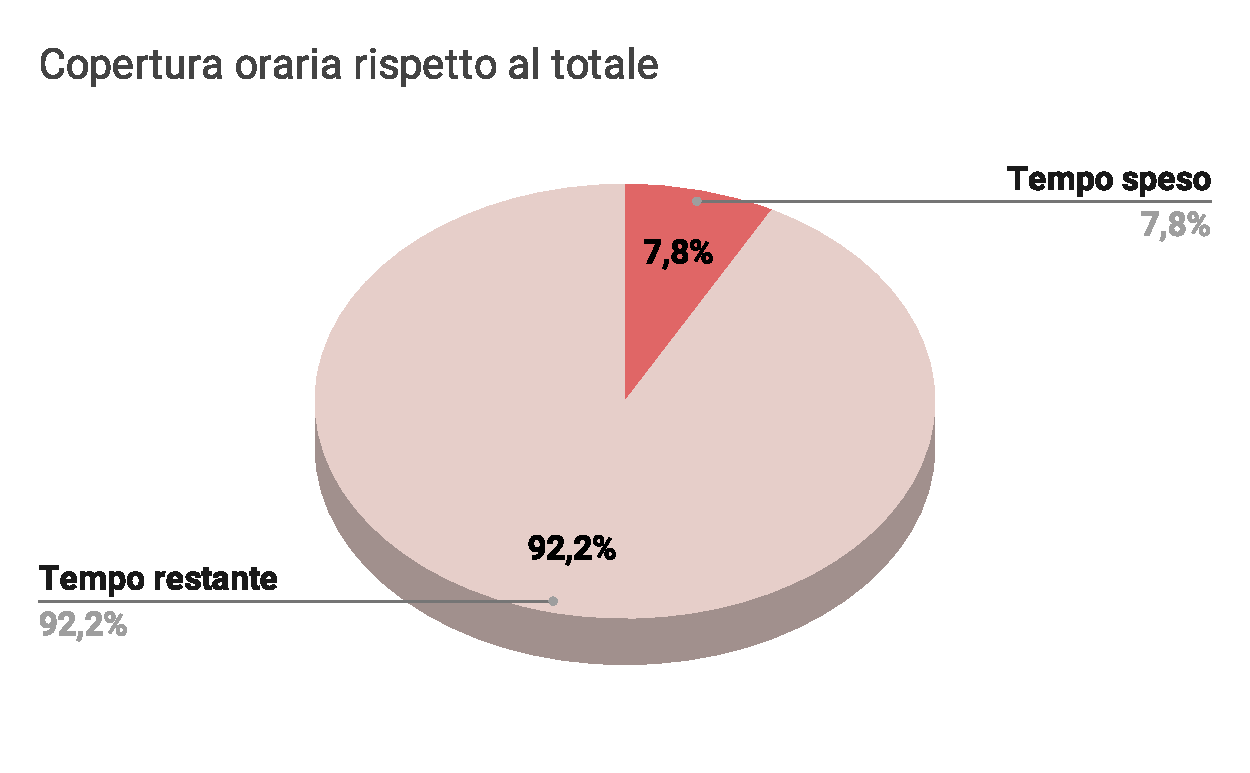
\includegraphics[width=0.90\textwidth]{assets/Consuntivo/Sprint-1/copertura_oraria.pdf}
  \caption{Sprint 1 - Areogramma del tempo speso (in ore) rispetto al totale}
\end{figure}

\begin{figure}[H]
  \centering
  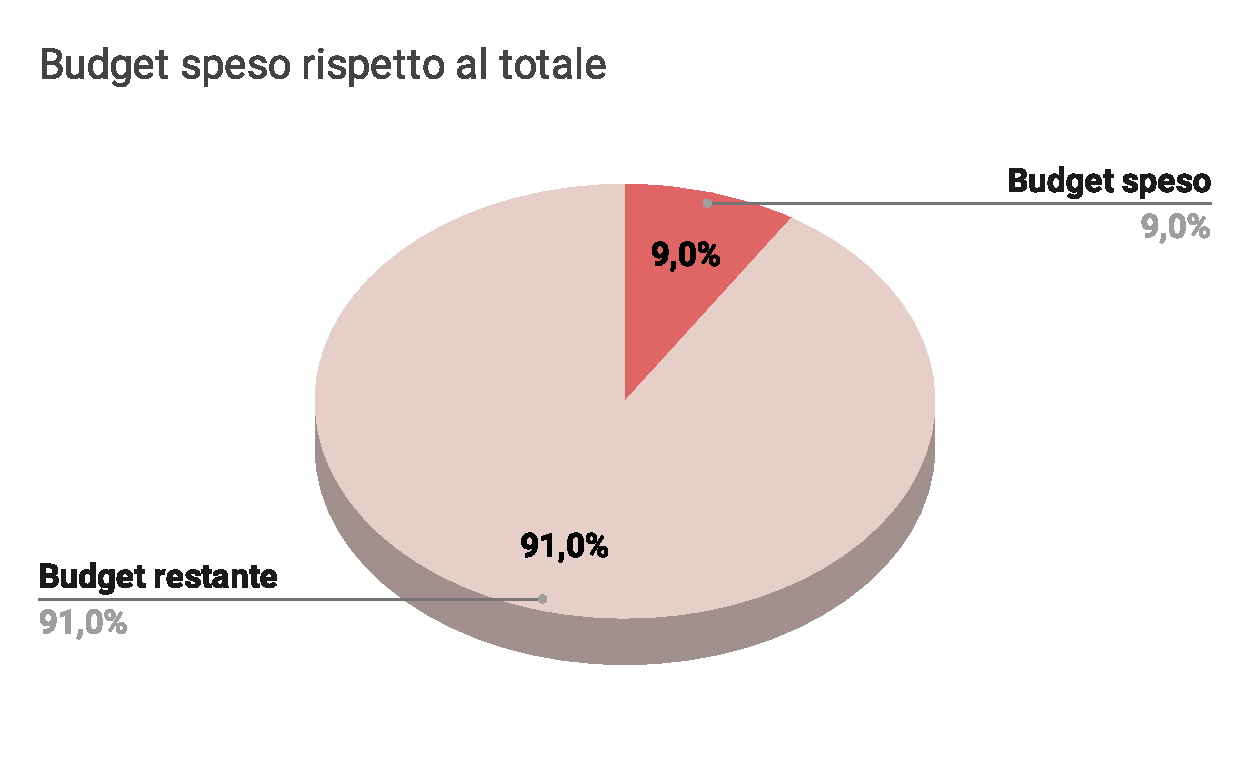
\includegraphics[width=0.90\textwidth]{assets/Consuntivo/Sprint-1/budget_speso.pdf}
  \caption{Sprint 1 - Areogramma del budget speso rispetto al totale}
\end{figure}


\begin{minipage}{\textwidth}
  Di seguito sono riportate le ore rimanenti per la coppia risorsa-ruolo:
  \begin{table}[H]
    \begin{tabularx}{\textwidth}{|c|*{6}{>{\centering}X|}c|}
      \hline
      \multicolumn{8}{|c|}{\textbf{Ore rimanenti per la coppia risorsa-ruolo}} \\
      \hline
      \textbf{Membro del team} & \textbf{Re} & \textbf{Am} & \textbf{An} & \textbf{Pt} & \textbf{Pr} & \textbf{Ve} & \textbf{Totale per persona} \\
      \hline
      Cavalli Riccardo & 2 & 8 & 9 & 23 & 22 & 20 & 84 \\
      \hline
      Pianon Raul & 9 & 8 & 9 & 23 & 22 & 12 & 83 \\
      \hline
      Dall'Amico Martina & 9 & 8 & 1 & 23 & 22 & 20 & 83 \\
      \hline
      Cristo Marco & 9 & 8 & 2 & 23 & 22 & 20 & 84 \\
      \hline
      Lewental Sebastiano & 9 & 8 & 2 & 23 & 22 & 20 & 84 \\
      \hline
      Zecchinato Mattia & 9 & 8 & 8 & 17 & 22 & 20 & 84 \\
      \hline
      Stocco Tommaso & 9 & 2 & 9 & 23 & 22 & 20 & 85 \\
      \hline
      \textbf{Totale per ruolo} & 56 & 50 & 40 & 155 & 154 & 132 & \textbf{587} \\
      \hline
    \end{tabularx}
    \caption{Sprint 1 - Ore rimanenti per la coppia risorsa-ruolo}
  \end{table}
  \end{minipage}

\subsubsection{Revisione delle attività}

Nel corso del primo \glossario{sprint}, il team ha svolto le seguenti attività:
\begin{itemize}
  \item Stesura iniziale del \PdP;
  \item Scelta del modello di sviluppo;
  \item Pianificazione e preventivo del secondo \glossario{sprint};
  \item \AdR\ e definizione dei primi \glossario{casi d'uso};
  \item Individuazione degli \glossario{attori} coinvolti nel sistema e delle loro caratteristiche;
  \item Analisi dei rischi tecnologici e organizzativi;
  \item Progettazione del \glossario{dizionario dati};
  \item Raccolta dei termini da inserire nel \Gls;
  \item Miglioramento del \WoW\ e automazione delle procedure con relativa stesura delle \NdP.
\end{itemize}

\subsubsection{Retrospettiva}

\par Di seguito sono riportati i risultati del questionario di valutazione dello \glossario{sprint}, realizzato dal Responsabile in carica per ottimizzare la fase di \glossario{retrospettiva}:
\begin{itemize}
  \item Organizzazione dello \glossario{sprint} - Valutazione: 7,5;
  \item Conduzione dei meeting interni - Valutazione: 7,5;
  \item Conduzione dei meeting esterni - Valutazione: 8;
  \item Impegno e partecipazione dei singoli membri - Valutazione: 7;
  \item Non tutti i membri del team erano a conoscenza delle proprie mansioni;
  \item La numerosità delle riunioni è adeguata;
  \item Le riunioni sono state organizzate quasi sempre con il giusto preavviso;
  \item Da migliorare il rapporto ore spese/ore produttive.
\end{itemize}

\subsubsection{Aggiornamento pianificazione e preventivo}
TODO

